\section{Mutual gravitational attraction of n-bodies}\label{sec:q1}

Given is:

%===========================================
\begin{equation}
    m_{i} \ddot{\bar{r_{i}}} = \sum_{j \neq i}^{} G \frac{m_{i}m_{j}}{r_{ij}^3} \bar{r_{ij}}
    \tag{2.3\cite{wakker}}
    \label{eq:grav_acc_i}
\end{equation}
%===========================================

\noindent \textbf{a) What is the meaning of the various parameters in \ref{eq:grav_acc_i}? Which fundamental laws have been used in the derivation of this equation?}

\bigskip

\noindent \textit{This question is discussed in \cite{wakker} page 25.}

\bigskip

\noindent The various parameters are:

%===========================================
\begin{itemize}
    \item $i$: body i
    \item $j$: body j
    \item $r_i$: position vector of body i (distance from the origin of the inertial reference frame XYZ to body i)
    \item $\ddot{\bar{r_i}}$: acceleration vector of body i
    \item $G$: Universal gravitational constant
    \item $m_i$: mass of body i
    \item $m_j$: mass of body j
    \item $r_{ij}$: distance from body i to body j
\end{itemize}
%===========================================

\noindent See Figure \ref{fig:grav_acc_i} for the representation of those parameters.

%===========================================
\begin{figure}[ht]
    \centering
    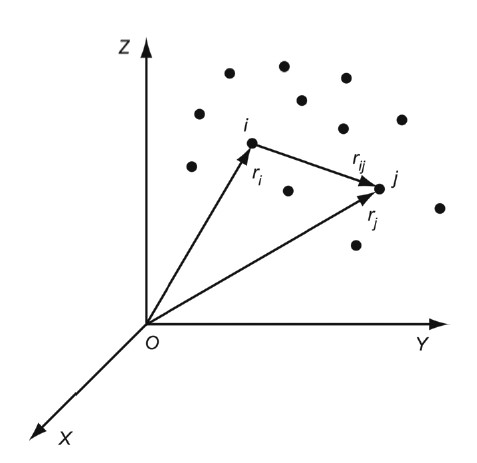
\includegraphics[width=6cm]{img/grav_acc.jpg}
    \caption{Position of n point masses relative to an inertial reference frame XYZ. \textit{This is Figure 2.1 in \cite{wakker}.}}
    \label{fig:grav_acc_i}
\end{figure}
%===========================================

\bigskip

\noindent The two fundamental laws used in the derivation of \ref{eq:grav_acc_i} are:

%===========================================
\begin{itemize}
    \item Newton's second law of motion
    \item Newton's law of gravitation
\end{itemize}
%===========================================

\newpage










\noindent \textbf{b) (i) Derive from \ref{eq:grav_acc_i} the following equation for the motion of body i relative to this reference frame.}

\bigskip

\noindent \textit{This derivation is performed in \cite{wakker} page 103-104.}

\bigskip

\noindent The motion of bodies i and k with respect to a non-rotating reference frame XYZ see Figure \ref{fig:grav_acc_2} with its origin at the center of mass of the n-body system (inertial reference frame) is written in Equations \ref{eq:grav_acc_i3} and \ref{eq:grav_acc_k3} for body i and k respectively.

%===========================================
\begin{figure}[ht]
    \centering
    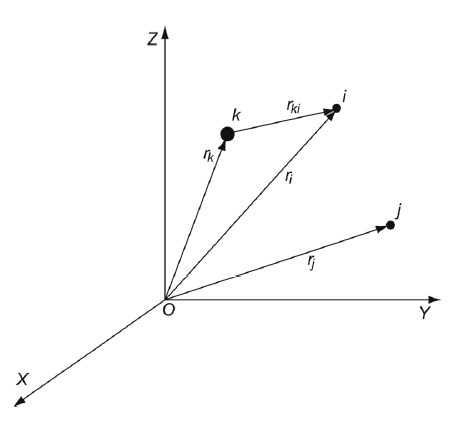
\includegraphics[width=7cm]{img/grav_acc2.jpg}
    \caption{Geometry of the bodies i, j and k relative to an inertial reference frame XYZ. \textit{This is Figure 4.1 in \cite{wakker}.}}
    \label{fig:grav_acc_2}
\end{figure}
%===========================================

\bigskip

\noindent For body i Equation \ref{eq:grav_acc_i} holds. Take out the the component of body k from the summation:

%===========================================
\begin{equation}
    m_{i} \ddot{\bar{r_{i}}} = G \frac{m_{i}m_{k}}{r_{ik}^3} \bar{r_{ik}} + \sum_{j \neq i,k}^{} G \frac{m_{i}m_{j}}{r_{ij}^3} \bar{r_{ij}}
    \label{eq:grav_acc_i2}
\end{equation}
%===========================================

\noindent Divide by $m_i$:

%===========================================
\begin{equation}
    \ddot{\bar{r_{i}}} = G \frac{m_{k}}{r_{ik}^3} \bar{r_{ik}} + \sum_{j \neq i,k}^{} G \frac{m_{j}}{r_{ij}^3} \bar{r_{ij}}
    \tag{4.2-1\cite{wakker}}
    \label{eq:grav_acc_i3}
\end{equation}
%===========================================

\noindent For body k holds:

%===========================================
\begin{equation}
    m_{k} \ddot{\bar{r_{k}}} = \sum_{j \neq k}^{} G \frac{m_{k}m_{j}}{r_{kj}^3} \bar{r_{kj}}
    \tag{4.1\cite{wakker}}
    \label{eq:grav_acc_k}
\end{equation}
%===========================================

\noindent Take out the the component of body i from the summation:

%===========================================
\begin{equation}
    m_{k} \ddot{\bar{r_{k}}} = G \frac{m_{k}m_{i}}{r_{ki}^3} \bar{r_{ki}} + \sum_{j \neq i,k}^{} G \frac{m_{k}m_{j}}{r_{kj}^3} \bar{r_{kj}}
    \label{eq:grav_acc_k2}
\end{equation}
%===========================================

\noindent Divide by $m_k$:

%===========================================
\begin{equation}
    \ddot{\bar{r_{k}}} = G \frac{m_{i}}{r_{ki}^3} \bar{r_{ki}} + \sum_{j \neq i,k}^{} G \frac{m_{j}}{r_{kj}^3} \bar{r_{kj}}
    \tag{4.2-2\cite{wakker}}
    \label{eq:grav_acc_k3}
\end{equation}
%===========================================

\noindent Subtract \ref{eq:grav_acc_k3} from \ref{eq:grav_acc_i3}:

%===========================================
\begin{equation}
    \ddot{\bar{r_{i}}} - \ddot{\bar{r_{k}}} = \Bigg[ G \frac{m_{k}}{r_{ik}^3} \bar{r_{ik}} - G \frac{m_{i}}{r_{ki}^3} \bar{r_{ki}} \Bigg] + \Bigg[ \sum_{j \neq i,k}^{} G \frac{m_{j}}{r_{ij}^3} \bar{r_{ij}} -\sum_{j \neq i,k}^{} G \frac{m_{j}}{r_{kj}^3} \bar{r_{kj}} \Bigg]
    \label{eq:grav_acc_subtr}
\end{equation}
%===========================================

\noindent Taking the following identities into account:

%===========================================
\begin{gather*}
    \bar{r_{ik}} = -\bar{r_{ki}}\\
    \bar{r_{ki}} = \bar{r_{i}} - \bar{r_{k}}\\
    \bar{r_{ij}} = \bar{r_{j}} - \bar{r_{i}} = \bar{r_{kj}} - \bar{r_{ki}}
    \tag{4.3\cite{wakker}}
    \label{eq:identities}
\end{gather*}
%===========================================

\noindent Applying \ref{eq:identities} to Equation \ref{eq:grav_acc_subtr}:

%===========================================
\begin{equation*}
    \boldsymbol{\ddot{\bar{r_{ki}}}} = \Bigg[ G \frac{m_{k}}{r_{ik}^3} (\boldsymbol{-\bar{r_{ki}}}) - G \frac{m_{i}}{r_{ki}^3} \bar{r_{ki}} \Bigg] + \Bigg[ \sum_{j \neq i,k}^{} G \frac{m_{j}}{r_{ij}^3} (\boldsymbol{\bar{r_{kj}} - \bar{r_{ki}}}) -\sum_{j \neq i,k}^{} G \frac{m_{j}}{r_{kj}^3} \bar{r_{kj}} \Bigg]
    \label{eq:grav_acc_subtr2}
\end{equation*}
%===========================================

%===========================================
\begin{equation}
    \ddot{\bar{r_{ki}}} = -G \frac{m_{i} + m_{k}}{r_{ki}^3} \bar{r_{ki}} + G\sum_{j \neq i,k}^{} m_{j} \Bigg( \frac{\bar{r_{j}} - \bar{r_{i}}}{r_{ij}^3} - \frac{\bar{r_{j}}}{r_{j}^3} \Bigg)
    \label{eq:grav_acc_subtr3}
\end{equation}
%===========================================

\noindent All vectors in this equation originate from body k. Now, the motion of body i with respect to a non-rotating reference frame fixed to body k is considered (as asked). This index k can consequently be omitted and Equation \ref{eq:grav_acc_subtr3} results in:

%===========================================
\begin{equation}
    \ddot{\bar{r_{i}}} = -G \frac{m_{i} + m_{k}}{r_{i}^3} \bar{r_{i}} + G\sum_{j \neq i,k}^{} m_{j} \Bigg( \frac{\bar{r_{j}} - \bar{r_{i}}}{r_{ij}^3} - \frac{\bar{r_{j}}}{r_{j}^3} \Bigg)
    \tag{4.4\cite{wakker}}
    \label{eq:grav_acc_subtr4}
\end{equation}
%===========================================










\noindent \textbf{b) (ii) Describe the physical meaning of the three terms on the right-hand side of Equation \ref{eq:grav_acc_subtr4}. Give a sketch in which the vectors $\bar{r_i}$ and $\bar{r_j}$ and the distance $r_{ij}$ are indicated.}

\bigskip

\noindent \textit{This question is discussed in \cite{wakker} page 32, 104 and 106.}

\bigskip

\noindent The first term of the right-hand side describes the two-body motion of body i about the barycenter, where the mass of body i and body k is assumed to be concentrated at the barycenter and only the gravitational attraction between the mass of body k and the mass of body i is accounted for.

\bigskip

\noindent The second term of the right-hand side expresses the acceleration of body i as a result of the gravitational attraction between body i and body j. This term is also described as the principal part.

\bigskip

\noindent The third term of the right-hand side expresses the acceleration of body k (i.e.  the origin of the reference frame) as a result of the gravitational attraction between bodies k and j. This term is also described as the indirect part.

\bigskip

\noindent The sketch is shown in the figure below.

%===========================================
\begin{figure}[ht]
    \centering
    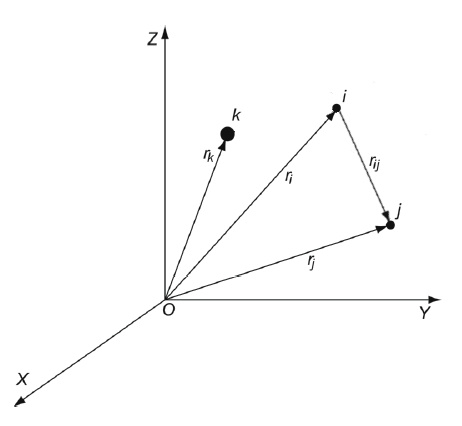
\includegraphics[width=7cm]{img/grav_acc3.jpg}
    \label{fig:grav_acc_3}
\end{figure}
%===========================================










\noindent \textbf{c) Derive from Equation \ref{eq:grav_acc_subtr4} the following relation for the main and disturbing accelerations of body i.}

\bigskip

\noindent \textit{This derivation is performed in \cite{wakker} page 104-108.}

\bigskip

\noindent The main acceleration of body i is only expressed by the first term of the right-hand side of Equation \ref{eq:grav_acc_subtr4}:

%===========================================
\begin{equation}
    \ddot{\bar{r_{m}}} = \bar{a_{m}} = -G \frac{m_{i} + m_{k}}{r_{i}^3} \bar{r_{i}} 
    \label{eq:grav_acc_c1}
\end{equation}
%===========================================

\noindent Now the magnitude of the main acceleration of body i is expressed. Note that the mass of body i is many times smaller than the mass of body k, thus it can be neglected. One can compare it, for example, with the mass of Earth w.r.t. the mass of the Sun or the mass of an artificial satellite w.r.t. the mass of the Earth. In other words $m_i << m_k$:

%===========================================
\begin{equation}
    a_{m} = G \frac{m_{i} + m_{k}}{r_{i}^3} \bar{r_{i}} \approx G \frac{m_{k}}{r_{i}^3} r_{i} = \boldsymbol{G\frac{m_{k}}{r_{i}^2}}
    \tag{4.9\cite{wakker}}
    \label{eq:grav_acc_c2}
\end{equation}
%===========================================

\noindent The perturbing acceleration is only expressed by the second and third term of the right-hand side of Equation \ref{eq:grav_acc_subtr4}. Note that body j is now expressed as body d:

%===========================================
\begin{equation}
    \ddot{\bar{r_{d}}} = \bar{a_{d}} = G m_{d} \Bigg( \frac{\bar{r_{d}} - \bar{r_{i}}}{r_{id}^3} - \frac{\bar{r_{d}}}{r_{d}^3} \Bigg) = G m_{d} \Bigg( \frac{\bar{r_{id}}}{r_{id}^3} - \frac{\bar{r_{d}}}{r_{d}^3} \Bigg)
    \label{eq:grav_acc_c3}
\end{equation}
%===========================================

\noindent Its magnitude is:

%===========================================
\begin{multline}
    a_{d} = G m_{d} \Bigg( \frac{\bar{r_{id}}}{r_{id}^3} - \frac{\bar{r_{d}}}{r_{d}^3} \Bigg) 
    = G m_{d} \sqrt{ \Bigg( \frac{\bar{r_{id}}}{r_{id}^3} - \frac{\bar{r_{d}}}{r_{d}^3} \Bigg) \Bigg( \frac{\bar{r_{id}}}{r_{id}^3} - \frac{\bar{r_{d}}}{r_{d}^3} \Bigg) } 
    = G m_{d} \sqrt{ \frac{r_{id}^2}{r_{id}^6} - \frac{\bar{r_{id}}\bar{r_{d}}}{r_{id}^3 r_{d}^3} - \frac{\bar{r_{d}}\bar{r_{id}}}{r_{d}^3 r_{id}^3} + \frac{r_{d}^2}{r_{d}^6}} \\
    = G m_{d} \sqrt{ \frac{1}{r_{id}^4} - 2\frac{\bar{r_{id}}\bar{r_{d}}}{r_{id}^3 r_{d}^3} + \frac{1}{r_{d}^4}} 
    = G m_{d} \sqrt{ \frac{1}{r_{id}^4} + \frac{1}{r_{d}^4} - 2\frac{\bar{r_{id}}\bar{r_{d}}}{r_{id}^3 r_{d}^3}}
    \tag{4.10\cite{wakker}}
    \label{eq:grav_acc_clong}
\end{multline}
%===========================================

\noindent It is known that:

%===========================================
\begin{equation}
    \bar{r_{id}}\bar{r_{d}} = r_{id} r_{d} \cos{\beta}
    \label{eq:grav_acc_c4}
\end{equation}
%===========================================

\noindent Using Figure \ref{fig:grav_acc_c1} below, $cos{\beta}$ becomes:

%===========================================
\begin{equation}
    \cos{\beta} = \frac{c}{r_{id}} = \frac{r_{d}-r_{i}\cos{\alpha}}{r_{id}} 
    \label{eq:grav_acc_c5}
\end{equation}
%===========================================

%===========================================
\begin{figure}[ht]
    \centering
    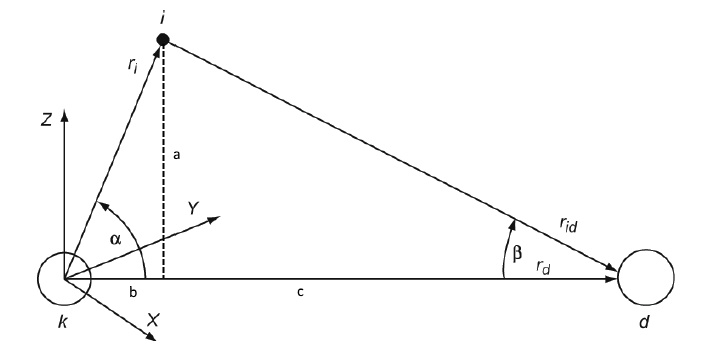
\includegraphics[width=10cm]{img/grav_acc_c1.jpg}
    \caption{Relative positions of bodies k, i and d. \textit{This is Figure 4.2 in \cite{wakker}.}}
    \label{fig:grav_acc_c1}
\end{figure}
%===========================================

\noindent Using Equations \ref{eq:grav_acc_c4} and \ref{eq:grav_acc_c5}, Equation \ref{eq:grav_acc_clong} becomes:

%===========================================
\begin{multline}
    a_{d} = G m_{d} \sqrt{ \frac{1}{r_{id}^4} + \frac{1}{r_{d}^4} - 2\frac{ \boldsymbol{r_{id} r_{d} \cos{\beta}} }{r_{id}^3 r_{d}^3}} = G m_{d} \sqrt{ \frac{1}{r_{id}^4} + \frac{1}{r_{d}^4} - 2\frac{\cos{\beta}}{r_{id}^2 r_{d}^2}} = G m_{d} \sqrt{\frac{1}{r_{id}^4} + \frac{1}{r_{d}^4} - 2\frac{\boldsymbol{(r_{d}-r_{i}\cos{\alpha})} }{r_{id}^{\boldsymbol{3}} r_{d}^2}} \\
    = G m_{d} \sqrt{\frac{1}{r_{id}^4}\boldsymbol{\frac{r_{d}^4}{r_{d}^4}} + \frac{1}{r_{d}^4} - 2\frac{(r_{d}-r_{i}\cos{\alpha}) }{r_{id}^3 r_{d}^2}\boldsymbol{\frac{r_{d}^2}{r_{d}^2}}} = G \frac{m_{d}}{r_{d}^2} \sqrt{\frac{r_{d}^4}{r_{id}^4} + 1 - 2\frac{(r_{d}-r_{i}\cos{\alpha}) r_{d}^2 }{r_{id}^3}}
    \label{eq:grav_acc_c6}
\end{multline}
%===========================================

\noindent For the common denominator $r_{id}$ (where applicable) inside the square root, using Figure \ref{fig:grav_acc_c1} and implementing the given relation $\gamma = \frac{r_{i}}{r_{d}}$, the denominator becomes:

%===========================================
\begin{equation}
    r_{id}^2 = (r_{i}^2 + r_{d}^2 - 2r_{i}r_{d}\cos{\alpha}) = \bigg[ r_{d}^2(\frac{r_{i}^2}{r_{d}^2} + 1 - 2\frac{r_{i}}{r_{d}}\cos{\alpha}) \bigg] = \bigg[ r_{d}^2(\gamma^2 + 1 - 2 \gamma\cos{\alpha}) \bigg]
    \label{eq:grav_acc_c7}
\end{equation}
%===========================================

\noindent Substituting Equation \ref{eq:grav_acc_c7} in Equation \ref{eq:grav_acc_c6}:

%===========================================
\begin{multline}
    a_{d} = G \frac{m_{d}}{r_{d}^2} \sqrt{\frac{r_{d}^4}{\boldsymbol{\bigg[ r_{d}^2(\gamma^2 + 1 - 2 \gamma\cos{\alpha}) \bigg]^2}} + 1 - 2\frac{(r_{d} - r_{i}\cos{\alpha}) r_{d}^2 }{\boldsymbol{\bigg[ r_{d}^2(\gamma^2 + 1 - 2 \gamma\cos{\alpha}) \bigg]^{3/2}}}} \\
    = G \frac{m_{d}}{r_{d}^2} \sqrt{\frac{\boldsymbol{r_{d}^4}}{ \boldsymbol{r_{d}^4}(\gamma^2 + 1 - 2 \gamma\cos{\alpha})^2} + 1 - 2\frac{(r_{d} - r_{i}\cos{\alpha}) \boldsymbol{r_{d}^2} }{\boldsymbol{r_{d}^3}(\gamma^2 + 1 - 2 \gamma\cos{\alpha})^{3/2}}} \\
    = G \frac{m_{d}}{r_{d}^2} \sqrt{\frac{1}{(\gamma^2 + 1 - 2 \gamma\cos{\alpha})^2} + 1 - 2\frac{(\boldsymbol{\frac{r_{d}}{r_{d}}} - \boldsymbol{\frac{r_{i}}{r_{d}}}\cos{\alpha}) }{(\gamma^2 + 1 - 2 \gamma\cos{\alpha})^{3/2}}} \\
    = G \frac{m_{d}}{r_{d}^2} \sqrt{\frac{1}{(\gamma^2 + 1 - 2 \gamma\cos{\alpha})^2} + 1 - 2\frac{(1 - \gamma\cos{\alpha}) }{(\gamma^2 + 1 - 2 \gamma\cos{\alpha})^{3/2}}} \\
    \label{eq:grav_acc_c8}
\end{multline}
%===========================================

\noindent Rearranging Equation \ref{eq:grav_acc_c8} gives the final result:

%===========================================
\begin{equation}
    a_{d} = G \frac{m_{d}}{r_{d}^2} \sqrt{1 + \frac{1}{(1 - 2 \gamma\cos{\alpha} + \gamma^2)^2} - \frac{2(1 - \gamma\cos{\alpha}) }{(1 - 2 \gamma\cos{\alpha} + \gamma^2)^{3/2}}}
    \tag{4.11\cite{wakker}}
    \label{eq:grav_acc_cfinal}
\end{equation}
%===========================================










\noindent \textbf{d) Derive from Equations \ref{eq:grav_acc_c2} and \ref{eq:grav_acc_cfinal} the following expression for the maximum relative perturbing acceleration of the satellite.}

\bigskip

\noindent \textit{This derivation is performed in \cite{wakker} page 108-109.}

\bigskip

\noindent For a maximum perturbing acceleration, angle $\alpha$ is zero degrees. Equation \ref{eq:grav_acc_cfinal} becomes:

%===========================================
\begin{multline}
    a_{d_{max}} = G \frac{m_{d}}{r_{d}^2} \sqrt{1 + \frac{1}{(1 - 2 \gamma + \gamma^2)^2} - \frac{2(1 - \gamma) }{(1 - 2 \gamma + \gamma^2)^{3/2}}} = G \frac{m_{d}}{r_{d}^2} \sqrt{1 + \frac{1}{((1 - \gamma)^2)^2} - \frac{2(1 - \gamma) }{((1 - \gamma)^2)^{3/2}}} \\
    = G \frac{m_{d}}{r_{d}^2} \sqrt{\boldsymbol{\frac{(1 - \gamma)^4}{(1 - \gamma)^4}} + \frac{1}{(1 - \gamma)^4} - \frac{2(1 - \gamma) }{(1 - \gamma)^3}\boldsymbol{\frac{(1 - \gamma)}{(1 - \gamma)}}}
    = G \frac{m_{d}}{r_{d}^2} \sqrt{\frac{\boldsymbol{(1 - \gamma)^4 + 1 - 2(1 - \gamma)^2}}{(1 - \gamma)^4}} \\
    = G \frac{m_{d}}{r_{d}^2} \sqrt{\frac{((1 - \gamma)^2 - 1)^2}{(1 - \gamma)^4}}
    = G \frac{m_{d}}{r_{d}^2} \Bigg[ \frac{((1 - \gamma)^2 - 1)}{(1 - \gamma)^2} \Bigg]
    = G \frac{m_{d}}{r_{d}^2} \Bigg[ \frac{(1 - \gamma)^2}{(1 - \gamma)^2} - \frac{1}{(1 - \gamma)^2} \Bigg] \\
    = G \frac{m_{d}}{r_{d}^2} \Bigg[ 1 - \frac{1}{(1 - \gamma)^2} \Bigg]
    = G \frac{m_{d}}{r_{d}^2} \Bigg| \frac{1}{(1 - \gamma)^2} - 1 \Bigg|
    = G \frac{m_{d}}{r_{d}^2} \Bigg| \Bigg( \frac{1}{1 - \gamma} \Bigg) ^2 - 1 \Bigg|
    \tag{4.14\cite{wakker}}
    \label{eq:grav_acc_d1}
\end{multline}
%===========================================

\noindent Divide Equation \ref{eq:grav_acc_d1} by Equation \ref{eq:grav_acc_c2}, replacing $\gamma$ with $\frac{r_{s}}{r_{d}}$, body k with Earth and body i with the satellite gives:

%===========================================
\begin{equation}
    \Bigg( \frac{a_{d}}{a_{m}} \Bigg)_{max} = \frac{G \frac{m_{d}}{r_{d}^2} \Big| \Big( \frac{1}{1 - \gamma} \Big) ^2 - 1 \Big| }{G\frac{m_{E}}{r_{s}^2}} = \frac{m_{d}}{m_{E}} \Bigg( \frac{r_{s}}{r_{d}} \Bigg)^2 \Bigg| \Bigg( \frac{1}{1 - \gamma} \Bigg) ^2 - 1 \Bigg| = \boldsymbol{\frac{m_{d}}{m_{E}} \Bigg( \frac{r_{s}}{r_{d}} \Bigg)^2 \Bigg| \Bigg( \frac{1}{1 - \frac{r_{s}}{r_{d}}} \Bigg) ^2 - 1 \Bigg|}
    \tag{4.13\cite{wakker}}
    \label{eq:grav_acc_d2}
\end{equation}
%===========================================










\noindent \textbf{e) Show that despite the large difference between the values of $m_d/m_E$, both the gravitational attraction by the Moon and the gravitational attraction by the Sun can be considered as a perturbation. Show that for both cases the following approximative expression holds for the maximum relative perturbing acceleration..}

\bigskip

\noindent \textit{This calculation is performed in \cite{wakker} page 109-111.}

\bigskip

\noindent With the given values and implementing those in Equation \ref{eq:grav_acc_d2} gives for the maximum relative perturbing acceleration:

%===========================================
\begin{itemize}
    \item Moon: $\big( \frac{a_{d}}{a_{m}} \big)_{max}$ = $1.7898\cdot10^{-7}$
    \item Sun: $\big( \frac{a_{d}}{a_{m}} \big)_{max}$ = $7.9881\cdot10^{-8}$
\end{itemize}
%===========================================

\noindent Both values are very small and thus the gravitational attraction of both the Moon and the Sun are perturbations.

\bigskip

\noindent Given is:

%===========================================
\begin{equation}
    \Bigg( \frac{a_{d}}{a_{m}} \Bigg)_{max} \approx 2 \frac{m_{d}}{m_{E}} \Bigg( \frac{r_{s}}{r_{d}} \Bigg) ^3
    \tag{4.16\cite{wakker}}
    \label{eq:grav_acc_d3}
\end{equation}
%===========================================

\bigskip

\noindent With the given values and implementing those in Equation \ref{eq:grav_acc_d3} gives for the maximum relative perturbing acceleration:

%===========================================
\begin{itemize}
    \item Moon: $\big( \frac{a_{d}}{a_{m}} \big)_{max}$ = $1.7384\cdot10^{-7}$
    \item Sun: $\big( \frac{a_{d}}{a_{m}} \big)_{max}$ = $7.98758\cdot10^{-8}$
\end{itemize}
%===========================================

\noindent These values are close to the ones calculated earlier, thus the approximative expression holds for the maximum relative perturbing acceleration.